\documentclass[11pt]{article}
\usepackage[margin=1in]{geometry}
\usepackage{booktabs}
\usepackage{longtable}
\usepackage{array}
\usepackage{amsmath}
\usepackage{graphicx}
\usepackage[section]{placeins}
\usepackage{hyperref}
\hypersetup{colorlinks=true, linkcolor=blue, urlcolor=blue}
\sloppy
\newcolumntype{L}[1]{>{\raggedright\arraybackslash}p{#1}}

% Every number in this document is defined by analyze_permit_content.py (`clocks') in the
% generated files under tables/. Nothing is typed by hand.
% GENERATED BY analyze_permit_content.py clocks --- do not edit by hand.
\newcommand{\ckAppHearingCvCu}{1.32}
\newcommand{\ckAppHearingCvDr}{1.27}
\newcommand{\ckAppHearingCvLpa}{1.12}
\newcommand{\ckAppHearingMedCu}{161}
\newcommand{\ckAppHearingMedDr}{301}
\newcommand{\ckAppHearingMedLpa}{603}
\newcommand{\ckAppHearingNCu}{3{,}141}
\newcommand{\ckAppHearingNDr}{2{,}311}
\newcommand{\ckAppHearingNLpa}{141}
\newcommand{\ckAppHearingNegCu}{6}
\newcommand{\ckAppHearingNegDr}{67}
\newcommand{\ckAppHearingNegLpa}{3}
\newcommand{\ckClockFrom}{1998}
\newcommand{\ckCvHiCu}{0.81}
\newcommand{\ckCvHiDr}{0.58}
\newcommand{\ckCvHiLpa}{---}
\newcommand{\ckCvHiMin}{0.98}
\newcommand{\ckCvLoCu}{0.67}
\newcommand{\ckCvLoDr}{0.71}
\newcommand{\ckCvLoLpa}{---}
\newcommand{\ckCvLoMin}{0.86}
\newcommand{\ckCvRhoCu}{0.10}
\newcommand{\ckCvRhoDr}{-0.40}
\newcommand{\ckCvRhoLpa}{---}
\newcommand{\ckCvRhoMin}{0.30}
\newcommand{\ckFiledIssuedCvCu}{1.19}
\newcommand{\ckFiledIssuedCvDr}{0.82}
\newcommand{\ckFiledIssuedCvLpa}{0.93}
\newcommand{\ckFiledIssuedCvMin}{1.08}
\newcommand{\ckFiledIssuedMedCu}{434}
\newcommand{\ckFiledIssuedMedDr}{631}
\newcommand{\ckFiledIssuedMedLpa}{722}
\newcommand{\ckFiledIssuedMedMin}{338}
\newcommand{\ckFiledIssuedNCu}{1{,}436}
\newcommand{\ckFiledIssuedNDr}{2{,}311}
\newcommand{\ckFiledIssuedNLpa}{115}
\newcommand{\ckFiledIssuedNMin}{28{,}498}
\newcommand{\ckFiledIssuedNegCu}{0}
\newcommand{\ckFiledIssuedNegDr}{1}
\newcommand{\ckFiledIssuedNegLpa}{0}
\newcommand{\ckFiledIssuedNegMin}{0}
\newcommand{\ckFinalIssuedCvCu}{1.88}
\newcommand{\ckFinalIssuedCvDr}{2.06}
\newcommand{\ckFinalIssuedCvLpa}{1.37}
\newcommand{\ckFinalIssuedMedCu}{408}
\newcommand{\ckFinalIssuedMedDr}{230}
\newcommand{\ckFinalIssuedMedLpa}{700}
\newcommand{\ckFinalIssuedNCu}{1{,}328}
\newcommand{\ckFinalIssuedNDr}{2{,}088}
\newcommand{\ckFinalIssuedNLpa}{94}
\newcommand{\ckFinalIssuedNegCu}{90}
\newcommand{\ckFinalIssuedNegDr}{70}
\newcommand{\ckFinalIssuedNegLpa}{4}
\newcommand{\ckFirstFinalPctCu}{73}
\newcommand{\ckFirstFinalPctDr}{68}
\newcommand{\ckFirstFinalPctLpa}{75}
\newcommand{\ckFirstFinalPctMin}{---}
\newcommand{\ckHearingFinalCvCu}{3.52}
\newcommand{\ckHearingFinalCvDr}{2.51}
\newcommand{\ckHearingFinalCvLpa}{3.02}
\newcommand{\ckHearingFinalMedCu}{0}
\newcommand{\ckHearingFinalMedDr}{0}
\newcommand{\ckHearingFinalMedLpa}{0}
\newcommand{\ckHearingFinalNCu}{3{,}205}
\newcommand{\ckHearingFinalNDr}{2{,}467}
\newcommand{\ckHearingFinalNLpa}{150}
\newcommand{\ckHearingFinalNegCu}{0}
\newcommand{\ckHearingFinalNegDr}{0}
\newcommand{\ckHearingFinalNegLpa}{0}
\newcommand{\ckHorizon}{5{,}500}
\newcommand{\ckIqrRhoCu}{---}
\newcommand{\ckIqrRhoDr}{---}
\newcommand{\ckIqrRhoLpa}{---}
\newcommand{\ckIqrRhoMin}{---}
\newcommand{\ckIssuedDoneCvCu}{1.02}
\newcommand{\ckIssuedDoneCvDr}{0.87}
\newcommand{\ckIssuedDoneCvLpa}{0.49}
\newcommand{\ckIssuedDoneCvMin}{0.98}
\newcommand{\ckIssuedDoneMedCu}{762}
\newcommand{\ckIssuedDoneMedDr}{759}
\newcommand{\ckIssuedDoneMedLpa}{1{,}307}
\newcommand{\ckIssuedDoneMedMin}{642}
\newcommand{\ckIssuedDoneNCu}{1{,}117}
\newcommand{\ckIssuedDoneNDr}{1{,}912}
\newcommand{\ckIssuedDoneNLpa}{90}
\newcommand{\ckIssuedDoneNMin}{22{,}233}
\newcommand{\ckIssuedDoneNegCu}{3}
\newcommand{\ckIssuedDoneNegDr}{2}
\newcommand{\ckIssuedDoneNegLpa}{0}
\newcommand{\ckIssuedDoneNegMin}{7}
\newcommand{\ckMature}{2013}
\newcommand{\ckMinCell}{20}
\newcommand{\ckPermitCvHiCu}{1.23}
\newcommand{\ckPermitCvHiDr}{0.88}
\newcommand{\ckPermitCvHiLpa}{---}
\newcommand{\ckPermitCvHiMin}{1.13}
\newcommand{\ckPermitCvLoCu}{1.12}
\newcommand{\ckPermitCvLoDr}{0.99}
\newcommand{\ckPermitCvLoLpa}{---}
\newcommand{\ckPermitCvLoMin}{1.18}
\newcommand{\ckPermitCvRhoCu}{0.10}
\newcommand{\ckPermitCvRhoDr}{-0.10}
\newcommand{\ckPermitCvRhoLpa}{---}
\newcommand{\ckPermitCvRhoMin}{-0.60}
\newcommand{\ckPermitPctCu}{45}
\newcommand{\ckPermitPctDr}{94}
\newcommand{\ckPermitPctLpa}{77}
\newcommand{\ckPermitPctMin}{100}
\newcommand{\ckRetrieved}{2026-09-11}
\newcommand{\ckTotCvCu}{0.79}
\newcommand{\ckTotCvDr}{0.67}
\newcommand{\ckTotCvLpa}{0.52}
\newcommand{\ckTotCvMin}{0.95}
\newcommand{\ckTotIqrCu}{---}
\newcommand{\ckTotIqrDr}{---}
\newcommand{\ckTotIqrLpa}{1.26}
\newcommand{\ckTotIqrMin}{---}
\newcommand{\ckTotMatNCu}{423}
\newcommand{\ckTotMatNDr}{955}
\newcommand{\ckTotMatNLpa}{40}
\newcommand{\ckTotMatNMin}{9{,}373}
\newcommand{\ckTotMedCu}{2{,}232}
\newcommand{\ckTotMedDr}{1{,}817}
\newcommand{\ckTotMedLpa}{3{,}394}
\newcommand{\ckTotMedMin}{1{,}334}
\newcommand{\ckTotPninetyCu}{---}
\newcommand{\ckTotPninetyDr}{---}
\newcommand{\ckTotPninetyLpa}{---}
\newcommand{\ckTotPninetyMin}{---}
\newcommand{\ckTotStenPctCu}{36}
\newcommand{\ckTotStenPctDr}{34}
\newcommand{\ckTotStenPctLpa}{48}
\newcommand{\ckTotStenPctMin}{34}
\newcommand{\ckTotalCvCu}{0.76}
\newcommand{\ckTotalCvDr}{0.64}
\newcommand{\ckTotalCvLpa}{0.50}
\newcommand{\ckTotalCvMin}{0.80}
\newcommand{\ckTotalMedCu}{2{,}232}
\newcommand{\ckTotalMedDr}{1{,}817}
\newcommand{\ckTotalMedLpa}{3{,}394}
\newcommand{\ckTotalMedMin}{1{,}334}
\newcommand{\ckTotalNCu}{1{,}440}
\newcommand{\ckTotalNDr}{2{,}311}
\newcommand{\ckTotalNLpa}{115}
\newcommand{\ckTotalNMin}{28{,}498}
\newcommand{\ckTotalNegCu}{0}
\newcommand{\ckTotalNegDr}{1}
\newcommand{\ckTotalNegLpa}{0}
\newcommand{\ckTotalNegMin}{7}
\newcommand{\ckUnitsCu}{3{,}205}
\newcommand{\ckUnitsDr}{2{,}467}
\newcommand{\ckUnitsLpa}{150}
\newcommand{\ckUnitsMin}{28{,}498}
\newcommand{\ckValueCover}{87.8}
\newcommand{\ckValueQ}{5}
\newcommand{\ckValuedLater}{14{,}593}

% GENERATED BY analyze_permit_content.py outcomes --- do not edit by hand.
\newcommand{\ocCifCu}{68}
\newcommand{\ocCifDr}{68}
\newcommand{\ocCifExitCu}{16}
\newcommand{\ocCifExitDr}{20}
\newcommand{\ocCifExitLpa}{7}
\newcommand{\ocCifExitMin}{28}
\newcommand{\ocCifLpa}{64}
\newcommand{\ocCifMin}{56}
\newcommand{\ocDoneCu}{79}
\newcommand{\ocDoneDr}{78}
\newcommand{\ocDoneHiCu}{77}
\newcommand{\ocDoneHiDr}{70}
\newcommand{\ocDoneHiMin}{60}
\newcommand{\ocDoneHp}{60}
\newcommand{\ocDoneLoCu}{81}
\newcommand{\ocDoneLoDr}{70}
\newcommand{\ocDoneLoMin}{65}
\newcommand{\ocDoneLpa}{94}
\newcommand{\ocDoneMin}{63}
\newcommand{\ocExitCu}{17}
\newcommand{\ocExitDr}{16}
\newcommand{\ocExitLpa}{3}
\newcommand{\ocExitMin}{28}
\newcommand{\ocFcdCover}{46}
\newcommand{\ocIssuedCu}{87}
\newcommand{\ocIssuedDr}{91}
\newcommand{\ocIssuedLpa}{97}
\newcommand{\ocIssuedMin}{75}
\newcommand{\ocMature}{2{,}136}
\newcommand{\ocMatureFrom}{2005}
\newcommand{\ocMatureTo}{2014}
\newcommand{\ocMedYearsCu}{3.7}
\newcommand{\ocMedYearsDr}{2.6}
\newcommand{\ocMedYearsLpa}{4.1}
\newcommand{\ocMedYearsMin}{2.8}
\newcommand{\ocNCu}{141}
\newcommand{\ocNDr}{171}
\newcommand{\ocNLpa}{33}
\newcommand{\ocNMin}{1{,}791}
\newcommand{\ocNeverCu}{32}
\newcommand{\ocNeverDr}{32}
\newcommand{\ocNeverLpa}{36}
\newcommand{\ocNeverMin}{44}
\newcommand{\ocOpenCu}{4}
\newcommand{\ocOpenDr}{6}
\newcommand{\ocOpenLpa}{3}
\newcommand{\ocOpenMin}{9}
\newcommand{\ocUnits}{10{,}253}
\newcommand{\ocUnitsApprCu}{6{,}583}
\newcommand{\ocUnitsApprDr}{386}
\newcommand{\ocUnitsApprLpa}{4{,}037}
\newcommand{\ocUnitsApprMin}{18{,}531}
\newcommand{\ocUnitsHpCu}{5{,}532}
\newcommand{\ocUnitsHpDr}{314}
\newcommand{\ocUnitsHpLpa}{3{,}952}
\newcommand{\ocUnitsHpMin}{8{,}715}
\newcommand{\ocUnitsShareCu}{84}
\newcommand{\ocUnitsShareDr}{81}
\newcommand{\ocUnitsShareLpa}{98}
\newcommand{\ocUnitsShareMin}{47}
\newcommand{\ocYears}{10}


\title{The Clocks:\\
\large the full distribution of every duration, by track and parcel value}
\author{Dan Post}
\date{September 2026}

\begin{document}
\maketitle

\begin{abstract}
\noindent
The model separates a deterministic cost from uncertainty, and the uncertainty channel is
identified by dispersion: a level alone cannot tell the two apart. The earlier memos reported
means and medians. This memo reports, for every clock the project measures --- application to
first hearing, first hearing to final action, permit filing to issuance, final action to
issuance, issuance to completion, and the developer's whole clock from first filing to
completion --- the full distribution, by track, and handles right-censoring with
Kaplan--Meier estimates so that recent cohorts count.

\medskip\noindent
\textbf{The developer's clock is long and dispersed on every track.} Its Kaplan--Meier median
is \ckTotMedCu\ days for conditional use, \ckTotMedDr\ for discretionary review, \ckTotMedLpa\
for large project authorisations and \ckTotMedMin\ for development permits that never reach
the Commission. Among cohorts first filed before \ckMature, whose spells have had a decade to
finish, the coefficient of variation of the completed clock is \ckTotCvCu, \ckTotCvDr,
\ckTotCvLpa\ and \ckTotCvMin.

\medskip\noindent
\textbf{About a third of spells never record a completion.} Ten years after first filing,
\ckTotStenPctCu\%, \ckTotStenPctDr\%, \ckTotStenPctLpa\% and \ckTotStenPctMin\% of spells on the
four tracks are still open. The survival curves therefore never reach their upper quartile,
and the upper tail of the developer's clock --- where dispersion lives --- is not observed; it
is truncated by non-completion, not only by censoring.

\medskip\noindent
\textbf{Dispersion does not fall consistently with parcel value.} Across city-wide quintiles of assessed
value per square foot, the CV of the completed developer's clock goes from \ckCvLoCu\ to
\ckCvHiCu\ on the conditional-use track (rank correlation \ckCvRhoCu), from \ckCvLoDr\ to
\ckCvHiDr\ on the DR track (\ckCvRhoDr), and from \ckCvLoMin\ to \ckCvHiMin\ off the Commission
(\ckCvRhoMin). A CV falling with value would be the wedge's signature. These moments do not
show it; they are descriptions, and they do not rule it out.

\medskip\noindent
\textbf{The hearing is rarely where the time goes.} \ckFirstFinalPctCu\% of conditional uses
and \ckFirstFinalPctDr\% of DRs are decided at their first hearing; the waits that carry the
dispersion are before the hearing and after it, in the permit.
\end{abstract}

\clearpage
\tableofcontents
\newpage

% ═══════════════════════════════════════════════════════════════════════════
\section{What this memo measures, and why it is a memo of its own}

The brief allowed either a new memo or a section of the permits memo. It is a memo of its own
because its object is different: the permits memo asks whether projects that reach the
Commission differ from similar projects that do not, and answers with means compared within
cells; this memo asks for the whole distribution of each duration --- the moments a model with
an uncertainty channel is estimated on --- and its unit of observation, for the Commission
tracks, is the case rather than the permit. The code is a stage of the permit-content pipeline
(\texttt{analyze\_permit\_content.py clocks}), which it shares its permit table, linkage tiers
and development-relevant universe with.

\paragraph{Tracks.} A \emph{Commission track} is a case --- a case number in the item table ---
whose first hearing was on a conditional use (including its modification), a discretionary
review, or a large project authorisation. The \emph{ministerial or by-right track} is the
development-relevant permits (the permits memo's universe) that no linkage tier connects to the
Commission, filed from \ckClockFrom, when the corpus begins; earlier permits that never
recorded a completion would otherwise sit ``at risk'' for decades and hold up every survival
curve. These are \ckUnitsCu\ conditional-use cases, \ckUnitsDr\ DR cases, \ckUnitsLpa\ large
project authorisations and \ckUnitsMin\ ministerial permits.

\paragraph{The permit a case's clock runs through.} A case reaches DBI through the permits
memo's tiers T1 (a permit number printed in the minutes) and T2 (the Planning records' permit
field). On the DR track the clock runs through the permit under review --- the earliest-filed
linked permit, as in the permits memo's DR clock. Otherwise it runs through the project's main
permit: new construction first, then a site permit, then the largest estimated cost. A case
with no linked permit has no permit clock at all (missing, not censored): \ckPermitPctCu\% of
conditional-use cases, \ckPermitPctDr\% of DRs and \ckPermitPctLpa\% of large project
authorisations have one. Many conditional uses are changes of use that need no
development permit.

\paragraph{The clocks.} Appendix~\ref{sec:defs} states each one's start and end. Two choices
matter. \emph{Application} is the opening of the earliest entitlement record for the case (the
data-acquisition memo's entitlement clock) except on the DR track, where it is the DBI filing of
the permit under review --- the developer's clock, not the neighbour's, as the note of
2026-09-11 in that memo now fixes by track. \emph{Final action} is the first hearing at which the
item table records a disposition that ends the case (approval, disapproval, taking or not taking
DR, withdrawal, adoption, certification, an appeal upheld); a continuance, an intent to approve
and ``no action'' do not.

\paragraph{Parcel value.} Assessed value (land plus improvements) per square foot of lot ---
of building where the roll records no lot area, as for condominium parcels --- in the roll year
nearest the first filing, binned into city-wide quintiles within that roll year; a case on
several parcels takes the median. \ckValueCover\% of units are valued. The assessor's roll
begins in 2007, so the \ckValuedLater\ units first filed earlier are valued at 2007. Proposition
13 holds assessed values at the acquisition price plus two percent a year, so the ranking is by
what was paid for a parcel as much as by what it is worth; the price surface in the
data-acquisition memo is the alternative, not used here.

% GENERATED BY analyze_permit_content.py clocks --- do not edit by hand.
\begin{table}[htbp]\centering
\caption{The units each track is measured on, and how many carry each clock. A spell counts when its start date exists; `done' is the share that has ended by the retrieval date; the rest are censored (still running, or the permit expired or was withdrawn).}\label{tab:inventory}
\resizebox{\textwidth}{!}{%
\begin{tabular}{lrrrrrrrrrrrrr}\toprule
Track & \multicolumn{2}{c}{application to first hearing} & \multicolumn{2}{c}{first hearing to final action} & \multicolumn{2}{c}{permit filed to issued} & \multicolumn{2}{c}{final action to permit issued} & \multicolumn{2}{c}{permit issued to completion} & \multicolumn{2}{c}{first filing to completion} & Units\\
\cmidrule(lr){2-3}\cmidrule(lr){4-5}\cmidrule(lr){6-7}\cmidrule(lr){8-9}\cmidrule(lr){10-11}\cmidrule(lr){12-13}
 & spells & done & spells & done & spells & done & spells & done & spells & done & spells & done & \\\midrule
conditional use & 3{,}141 & 100\% & 3{,}205 & 91\% & 1{,}436 & 78\% & 1{,}328 & 78\% & 1{,}117 & 68\% & 1{,}440 & 53\% & 3{,}205\\
discretionary review & 2{,}311 & 100\% & 2{,}467 & 90\% & 2{,}311 & 83\% & 2{,}088 & 85\% & 1{,}912 & 63\% & 2{,}311 & 53\% & 2{,}467\\
large project authorisation & 141 & 100\% & 150 & 81\% & 115 & 78\% & 94 & 77\% & 90 & 74\% & 115 & 58\% & 150\\
ministerial / by-right & 0 & --- & 0 & --- & 28{,}498 & 78\% & 0 & --- & 22{,}233 & 67\% & 28{,}498 & 53\% & 28{,}498\\
\bottomrule\end{tabular}}\end{table}


% ═══════════════════════════════════════════════════════════════════════════
\section{Censoring, and what it cannot fix}

A spell still running at the retrieval date (\ckRetrieved) is right-censored; so is a permit
spell that ends in expiry or withdrawal, censored at the exit. Reporting only completed spells
understates every duration for recent cohorts, because their long spells have not finished.
The Kaplan--Meier estimator counts each censored spell's exposure up to the point it was last
seen, and Figure~\ref{fig:km} draws it for every clock and track; Figure~\ref{fig:hazard} gives
the hazards of the permit clock and the developer's clock.

Censoring is not the only thing missing from the upper tail. Table~\ref{tab:inventory} shows
that only about half of the developer's clocks end in a recorded completion, and
Table~\ref{tab:headline} that a third of spells are still open ten years after first filing ---
far longer than any project is still under construction. Those spells are not running: they are
projects abandoned without an exit status, or completions DBI did not record. Kaplan--Meier
cannot tell a completion that was never recorded from one that has not happened, so for the
developer's clock its upper quartile is never reached (a dash in the tables) and the completed
spells of mature cohorts are the only view of the dispersion. The CV reported for the headline
is on those spells: cohorts first filed before \ckMature, which have had a decade to finish. It
describes the projects that finished, and says nothing about the ones that did not.

\begin{figure}[htbp]\centering
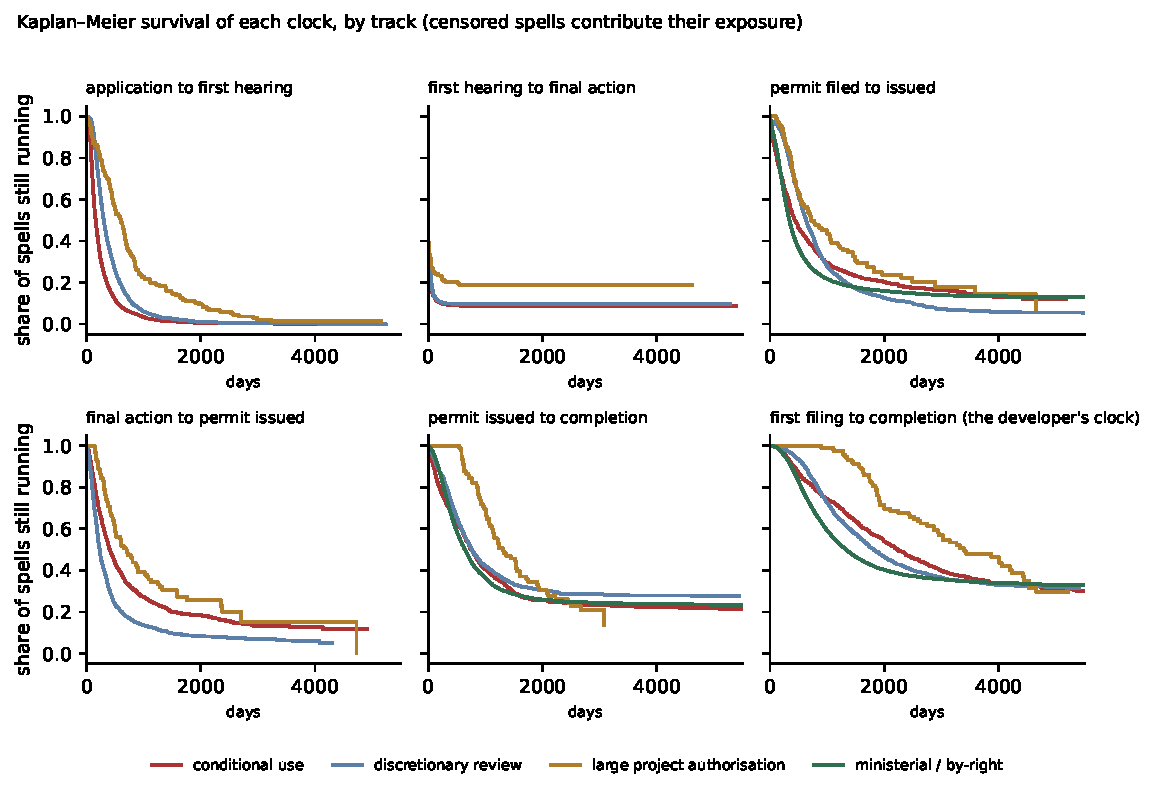
\includegraphics[width=\textwidth]{figures/fig_km.pdf}
\caption{Kaplan--Meier survival of each clock by track, drawn to \ckHorizon\ days. The legend
gives spells per track. The plateau in the second panel is cases with no final action in the
item table; in the last two, spells with no completion recorded.}
\label{fig:km}
\end{figure}

\begin{figure}[htbp]\centering
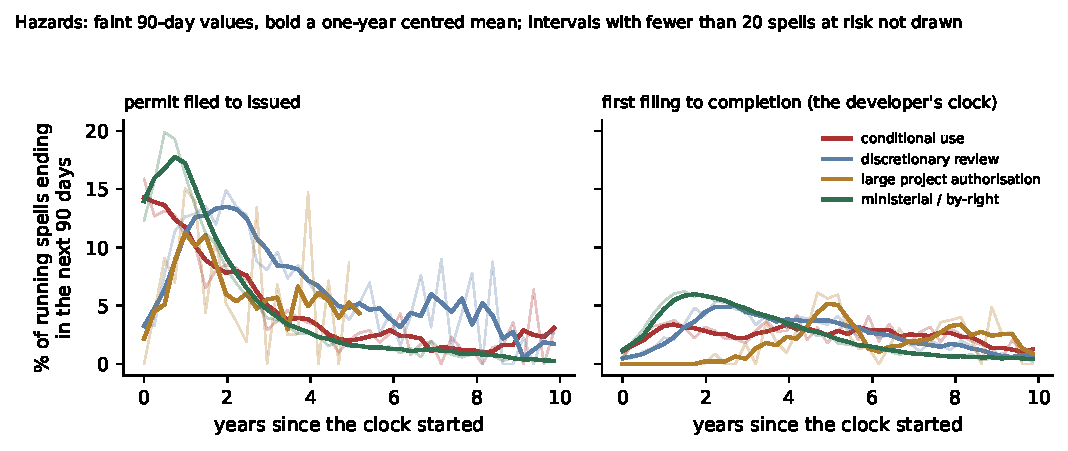
\includegraphics[width=\textwidth]{figures/fig_hazard.pdf}
\caption{Hazards of the permit clock and the developer's clock by track: the share of running
spells that end in the next 90 days.}
\label{fig:hazard}
\end{figure}

% ═══════════════════════════════════════════════════════════════════════════
\section{Every clock, by track}

Table~\ref{tab:moments} gives the distribution of every clock on every track: completed-spell
percentiles from the 10th to the 99th, the mean, the standard deviation of log days, the
coefficient of variation, and the Kaplan--Meier median and 90th percentile beside them.
Negative intervals are kept and counted, as in the earlier memos: they enter the quantiles and
the mean, and are left out only of the log-scale dispersion.

\begin{itemize}
\item \textbf{Application to first hearing} is the longest wait at the Commission and the most
dispersed: a Kaplan--Meier median of \ckAppHearingMedCu\ days on the conditional-use track (CV
\ckAppHearingCvCu), \ckAppHearingMedDr\ on the DR track (CV \ckAppHearingCvDr) --- where the
clock starts at the permit filing --- and \ckAppHearingMedLpa\ for large project authorisations.
\item \textbf{First hearing to final action} is short: \ckFirstFinalPctCu\% of conditional uses,
\ckFirstFinalPctDr\% of DRs and \ckFirstFinalPctLpa\% of large project authorisations are decided
at their first hearing. Its CV is high only because the distribution is a spike at zero with a
tail of continued cases.
\item \textbf{Permit filed to issued} has a median of \ckFiledIssuedMedCu, \ckFiledIssuedMedDr\
and \ckFiledIssuedMedLpa\ days on the three Commission tracks against \ckFiledIssuedMedMin\ off
it --- the permits memo's immortal-time caution applies: a permit reviewed at a hearing had to
survive to it.
\item \textbf{Final action to permit issued} carries negative intervals --- a permit issued
before the final action (\ckFinalIssuedNegCu\ conditional-use cases, \ckFinalIssuedNegDr\ DR
cases) --- which are kept.
\item \textbf{Permit issued to completion} and \textbf{the developer's clock} are the ones
non-completion truncates; see the previous section.
\end{itemize}

% GENERATED BY analyze_permit_content.py clocks --- do not edit by hand.
\begin{table}[htbp]\centering
\caption{Every clock, by track: the distribution of completed spells (days) --- percentiles, mean, the standard deviation of log days and the coefficient of variation --- beside the Kaplan--Meier median and 90th percentile, which count the censored spells' exposure. `Neg.' is the number of negative intervals, kept in every statistic except the log one. A dash: a cell under 20 observations, or a Kaplan--Meier quantile the curve never reaches.}\label{tab:moments}
\resizebox{\textwidth}{!}{%
\begin{tabular}{llrrrrrrrrrrrr}\toprule
Clock & Track & $n$ & Neg. & p10 & p25 & p50 & p75 & p90 & p99 & Mean & SD log & \textbf{CV} & KM p50 / p90\\\midrule
application to first hearing & conditional use & 3{,}141 & 6 & 63 & 94 & 161 & 301 & 549 & 1{,}681 & 266 & 0.85 & \textbf{1.32} & 161 / 552\\
 & discretionary review & 2{,}311 & 67 & 119 & 182 & 294 & 500 & 790 & 2{,}176 & 399 & 0.74 & \textbf{1.27} & 301 / 799\\
 & large project authorisation & 141 & 3 & 87 & 279 & 591 & 906 & 1{,}899 & 4{,}393 & 804 & 1.11 & \textbf{1.12} & 603 / 1{,}969\\
\midrule
first hearing to final action & conditional use & 2{,}932 & 0 & 0 & 0 & 0 & 7 & 55 & 322 & 20 & 1.09 & \textbf{3.52} & 0 / 224\\
 & discretionary review & 2{,}228 & 0 & 0 & 0 & 0 & 21 & 63 & 222 & 19 & 0.94 & \textbf{2.51} & 0 / 308\\
 & large project authorisation & 122 & 0 & 0 & 0 & 0 & 5 & 62 & 472 & 29 & 1.31 & \textbf{3.02} & 0 / ---\\
\midrule
permit filed to issued & conditional use & 1{,}116 & 0 & 27 & 118 & 316 & 655 & 1{,}126 & 2{,}900 & 490 & 1.39 & \textbf{1.19} & 434 / ---\\
 & discretionary review & 1{,}912 & 1 & 204 & 336 & 544 & 853 & 1{,}308 & 2{,}814 & 683 & 0.87 & \textbf{0.82} & 631 / 2{,}493\\
 & large project authorisation & 90 & 0 & 238 & 366 & 528 & 1{,}049 & 1{,}699 & 3{,}708 & 815 & 0.79 & \textbf{0.93} & 722 / 4{,}651\\
 & ministerial / by-right & 22{,}233 & 0 & 51 & 141 & 263 & 457 & 779 & 2{,}045 & 371 & 1.09 & \textbf{1.08} & 338 / ---\\
\midrule
final action to permit issued & conditional use & 1{,}042 & 90 & 33 & 112 & 270 & 530 & 962 & 2{,}353 & 342 & 1.00 & \textbf{1.88} & 408 / ---\\
 & discretionary review & 1{,}777 & 70 & 41 & 98 & 190 & 362 & 622 & 1{,}712 & 260 & 0.98 & \textbf{2.06} & 230 / 1{,}439\\
 & large project authorisation & 72 & 4 & 166 & 282 & 476 & 820 & 1{,}324 & 3{,}293 & 619 & 0.77 & \textbf{1.37} & 700 / 4{,}726\\
\midrule
permit issued to completion & conditional use & 763 & 3 & 64 & 155 & 432 & 839 & 1{,}331 & 2{,}593 & 596 & 1.30 & \textbf{1.02} & 762 / ---\\
 & discretionary review & 1{,}214 & 2 & 102 & 272 & 475 & 763 & 1{,}209 & 2{,}275 & 590 & 1.01 & \textbf{0.87} & 759 / ---\\
 & large project authorisation & 67 & 0 & 606 & 853 & 1{,}073 & 1{,}534 & 2{,}083 & 3{,}081 & 1{,}248 & 0.45 & \textbf{0.49} & 1{,}307 / ---\\
 & ministerial / by-right & 14{,}957 & 7 & 133 & 245 & 415 & 699 & 1{,}078 & 2{,}344 & 547 & 0.89 & \textbf{0.98} & 642 / ---\\
\midrule
first filing to completion & conditional use & 763 & 0 & 291 & 517 & 1{,}134 & 1{,}900 & 2{,}668 & 4{,}750 & 1{,}319 & 0.89 & \textbf{0.76} & 2{,}232 / ---\\
 & discretionary review & 1{,}214 & 1 & 441 & 684 & 1{,}035 & 1{,}617 & 2{,}210 & 3{,}899 & 1{,}231 & 0.72 & \textbf{0.64} & 1{,}817 / ---\\
 & large project authorisation & 67 & 0 & 1{,}353 & 1{,}734 & 1{,}995 & 3{,}292 & 4{,}438 & 6{,}629 & 2{,}624 & 0.46 & \textbf{0.50} & 3{,}394 / ---\\
 & ministerial / by-right & 14{,}970 & 7 & 271 & 440 & 707 & 1{,}122 & 1{,}656 & 3{,}416 & 879 & 0.75 & \textbf{0.80} & 1{,}334 / ---\\
\midrule
\bottomrule\end{tabular}}\end{table}


% ═══════════════════════════════════════════════════════════════════════════
\section{The headline: the developer's clock against parcel value}

The real-options frame predicts that uncertainty in delay and outcome raises a developer's
filing threshold and re-routes development toward higher-value parcels: uncertainty shifts the
threshold differently across parcel values, where a deterministic cost shifts it more nearly
uniformly. If the regulatory
process imposes more uncertainty on some parcels than others, the dispersion of the clock by
parcel value is where it would show first, and a CV falling with parcel value would be the
signature of the wedge. Table~\ref{tab:headline} and Figure~\ref{fig:dispersion} give the
developer's clock by track and value quintile.

The signature is not there. On the DR track the CV of the completed clock falls, loosely, from
\ckCvLoDr\ in the lowest quintile to \ckCvHiDr\ in the highest (rank correlation across the five
quintiles \ckCvRhoDr); on the conditional-use track it has no pattern (\ckCvLoCu\ to \ckCvHiCu,
\ckCvRhoCu); off the Commission it drifts up (\ckCvLoMin\ to \ckCvHiMin, \ckCvRhoMin). The permit
clock, which completes for most spells, does not line up with it track by track. Its CV goes from
\ckPermitCvLoCu\ to \ckPermitCvHiCu\ on the conditional-use track (\ckPermitCvRhoCu) and from
\ckPermitCvLoDr\ to \ckPermitCvHiDr\ on the DR track (\ckPermitCvRhoDr) --- no pattern on either
--- and from \ckPermitCvLoMin\ to \ckPermitCvHiMin\ off the Commission, where it falls
(\ckPermitCvRhoMin) while the developer's clock on the same track rose. A falling CV appears on
one clock of one track at a time, and the two clocks disagree on the ministerial track. The
large-project track has too few mature completions per quintile to say anything (\ckTotMatNLpa\
in all).

\textbf{This is a description, not an estimate, and it does not reject the prediction.} Four
things stand between these moments and the model's object. (i) The completed spells are the
projects that finished; if dispersion deters filing or causes abandonment on low-value parcels,
the high-dispersion projects there are the ones missing. (ii) Assessed value under Proposition
13 ranks parcels partly by when they last sold. (iii) The quintiles pool every period, and the
clock lengthened over time. (iv) The model's $\sigma$ is the dispersion a developer faces
\emph{ex ante}, conditional on what the developer knows; a cross-sectional CV mixes that with
the heterogeneity of the projects themselves --- size, type and neighbourhood, which the next
section cuts by, one at a time.

% GENERATED BY analyze_permit_content.py clocks --- do not edit by hand.
\begin{table}[htbp]\centering
\caption{\textbf{The developer's clock --- first filing to completion --- by track and parcel value.} Value is assessed value per square foot, city-wide quintile of the roll year (1 lowest). Left: Kaplan--Meier quantiles over every spell (days) and the interquartile range over the median; $S$(10 yr) is the share of spells still running ten years after first filing --- no completion recorded. Right: completed spells of cohorts first filed before 2013, which have had a decade to finish --- mean, coefficient of variation and standard deviation of log days. Descriptive: these are the moments, not estimates of anything.}\label{tab:headline}
\resizebox{\textwidth}{!}{%
\begin{tabular}{llrrrrrrrrrrr}\toprule
 & & & \multicolumn{6}{c}{Kaplan--Meier, all cohorts} & \multicolumn{4}{c}{Completed, first filed before 2013}\\
\cmidrule(lr){4-9}\cmidrule(lr){10-13}
Track & Value & Spells & p25 & Median & p75 & p90 & IQR/med. & $S$(10 yr) & $n$ & Mean & \textbf{CV} & SD log\\\midrule
conditional use & 1 & 196 & 1{,}021 & 2{,}421 & --- & --- & --- & 0.39 & 30 & 1{,}470 & \textbf{0.67} & 0.68\\
 & 2 & 220 & 860 & 2{,}691 & --- & --- & --- & 0.45 & 57 & 1{,}386 & \textbf{0.98} & 1.22\\
 & 3 & 228 & 825 & 2{,}181 & --- & --- & --- & 0.39 & 68 & 1{,}310 & \textbf{1.02} & 1.06\\
 & 4 & 317 & 1{,}066 & 2{,}338 & 5{,}303 & --- & 1.81 & 0.32 & 93 & 1{,}443 & \textbf{0.84} & 1.04\\
 & 5 & 288 & 759 & 2{,}231 & --- & --- & --- & 0.34 & 79 & 1{,}430 & \textbf{0.81} & 1.06\\
 & all & 1{,}440 & 960 & 2{,}232 & --- & --- & --- & 0.36 & 423 & 1{,}427 & \textbf{0.79} & 0.99\\
\midrule
discretionary review & 1 & 187 & 1{,}051 & 1{,}861 & --- & --- & --- & 0.37 & 68 & 1{,}148 & \textbf{0.71} & 0.91\\
 & 2 & 242 & 1{,}021 & 2{,}016 & --- & --- & --- & 0.36 & 93 & 1{,}271 & \textbf{0.63} & 0.66\\
 & 3 & 361 & 940 & 1{,}924 & --- & --- & --- & 0.33 & 155 & 1{,}164 & \textbf{0.62} & 0.58\\
 & 4 & 566 & 1{,}057 & 2{,}000 & --- & --- & --- & 0.38 & 208 & 1{,}158 & \textbf{0.76} & 0.89\\
 & 5 & 661 & 943 & 1{,}722 & --- & --- & --- & 0.35 & 257 & 1{,}012 & \textbf{0.58} & 0.62\\
 & all & 2{,}311 & 941 & 1{,}817 & --- & --- & --- & 0.34 & 955 & 1{,}113 & \textbf{0.67} & 0.71\\
\midrule
large project authorisation & 1 & 26 & 1{,}919 & 3{,}422 & --- & --- & --- & 0.47 & 5 & --- & \textbf{---} & ---\\
 & 2 & 24 & 2{,}519 & 4{,}055 & --- & --- & --- & 0.64 & 5 & --- & \textbf{---} & ---\\
 & 3 & 20 & 1{,}875 & 3{,}394 & 6{,}174 & 6{,}174 & 1.27 & 0.46 & 9 & --- & \textbf{---} & ---\\
 & 4 & 17 & --- & --- & --- & --- & --- & --- & --- & --- & \textbf{---} & ---\\
 & 5 & 12 & --- & --- & --- & --- & --- & --- & --- & --- & \textbf{---} & ---\\
 & all & 115 & 1{,}906 & 3{,}394 & 6{,}174 & --- & 1.26 & 0.48 & 40 & 2{,}846 & \textbf{0.52} & 0.48\\
\midrule
ministerial / by-right & 1 & 2{,}680 & 769 & 1{,}482 & --- & --- & --- & 0.36 & 592 & 815 & \textbf{0.86} & 0.82\\
 & 2 & 3{,}595 & 743 & 1{,}785 & --- & --- & --- & 0.41 & 907 & 842 & \textbf{1.02} & 0.79\\
 & 3 & 5{,}133 & 678 & 1{,}491 & --- & --- & --- & 0.38 & 1{,}540 & 774 & \textbf{0.90} & 0.68\\
 & 4 & 6{,}541 & 703 & 1{,}446 & --- & --- & --- & 0.36 & 1{,}957 & 813 & \textbf{0.89} & 0.67\\
 & 5 & 7{,}231 & 548 & 1{,}128 & --- & --- & --- & 0.33 & 2{,}657 & 629 & \textbf{0.98} & 0.71\\
 & all & 28{,}498 & 637 & 1{,}334 & --- & --- & --- & 0.34 & 9{,}373 & 764 & \textbf{0.95} & 0.75\\
\midrule
\bottomrule\end{tabular}}\end{table}


\begin{figure}[htbp]\centering
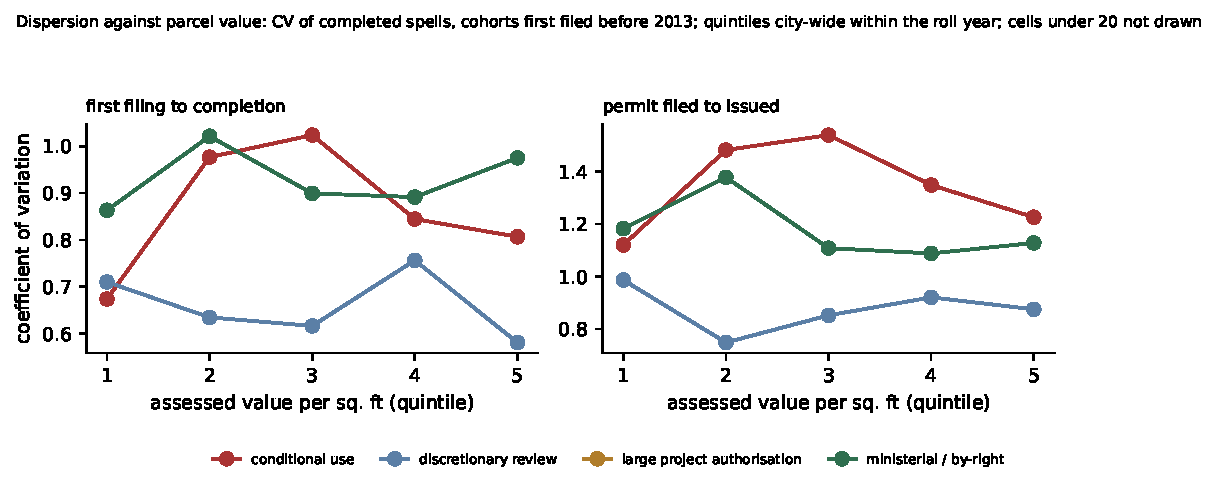
\includegraphics[width=\textwidth]{figures/fig_dispersion_value.pdf}
\caption{Coefficient of variation of completed spells by parcel-value quintile and track, for
cohorts first filed before \ckMature: the developer's clock (left) and the permit clock
(right).}
\label{fig:dispersion}
\end{figure}

% ═══════════════════════════════════════════════════════════════════════════
\section{The other cuts}

Tables~\ref{tab:byunitsPermit}--\ref{tab:byperiodTotal} and~\ref{tab:bynbhd} cut the permit
clock and the developer's clock by proposed units, by the five-year period of first filing, and
by the analysis neighbourhood of the project's permit. Every cell of every clock, with all the statistics of
Table~\ref{tab:moments}, is in \texttt{clock\_moments.csv} (\S\ref{sec:repro}); the tables here
show the Kaplan--Meier median and 90th percentile and the CV of completed spells, and omit cells
under \ckMinCell\ spells. By period the Kaplan--Meier medians of recent cohorts are computed on
short follow-up, and their 90th percentiles are mostly not yet reached.

% GENERATED BY analyze_permit_content.py clocks --- do not edit by hand.
\begin{table}[htbp]\centering
\caption{Permit filed to issued, by track and proposed units: spells, Kaplan--Meier median and 90th percentile (days), and the median and CV of completed spells. Cells under 20 spells omitted.}\label{tab:byunitsPermit}
\resizebox{\textwidth}{!}{%
\begin{tabular}{llrrrrrr}\toprule
Track & Proposed units & Spells & KM p50 & KM p90 & Done & p50 done & CV done\\\midrule
conditional use & 0 & 305 & 213 & --- & 248 & 164 & 1.20\\
 & 1 & 168 & 644 & --- & 122 & 457 & 1.11\\
 & 2--4 & 307 & 675 & --- & 241 & 478 & 0.96\\
 & 5--9 & 76 & 616 & --- & 59 & 376 & 1.15\\
 & 10--19 & 78 & 601 & 3{,}914 & 54 & 337 & 1.26\\
 & 20--49 & 124 & 535 & 3{,}420 & 97 & 355 & 1.20\\
 & 50+ & 171 & 482 & --- & 136 & 376 & 0.85\\
 & unknown & 207 & 273 & --- & 159 & 192 & 1.06\\
\midrule
discretionary review & 0 & 109 & 385 & --- & 73 & 239 & 1.07\\
 & 1 & 1{,}003 & 574 & 2{,}170 & 862 & 518 & 0.82\\
 & 2--4 & 681 & 709 & 2{,}675 & 551 & 623 & 0.75\\
 & 5--9 & 76 & 729 & --- & 53 & 498 & 0.84\\
 & 10--19 & 48 & 562 & 2{,}541 & 35 & 385 & 0.92\\
 & 20--49 & 44 & 663 & 2{,}892 & 36 & 598 & 0.84\\
 & 50+ & 29 & 336 & 1{,}002 & 25 & 302 & 0.56\\
 & unknown & 321 & 730 & 2{,}008 & 277 & 643 & 0.84\\
\midrule
large project authorisation & 20--49 & 21 & 1{,}071 & 4{,}651 & 18 & --- & ---\\
 & 50+ & 60 & 530 & --- & 51 & 463 & 0.65\\
\midrule
ministerial / by-right & 0 & 3{,}013 & 96 & 1{,}203 & 2{,}605 & 76 & 1.53\\
 & 1 & 11{,}065 & 334 & 3{,}427 & 9{,}068 & 285 & 0.96\\
 & 2--4 & 7{,}934 & 443 & --- & 5{,}741 & 321 & 0.94\\
 & 5--9 & 1{,}304 & 561 & --- & 918 & 394 & 0.92\\
 & 10--19 & 827 & 540 & --- & 601 & 386 & 0.90\\
 & 20--49 & 620 & 391 & --- & 437 & 248 & 1.02\\
 & 50+ & 910 & 198 & --- & 733 & 152 & 1.45\\
 & unknown & 2{,}825 & 286 & --- & 2{,}130 & 188 & 1.43\\
\midrule
\bottomrule\end{tabular}}\end{table}

% GENERATED BY analyze_permit_content.py clocks --- do not edit by hand.
\begin{table}[htbp]\centering
\caption{First filing to completion, by track and proposed units: spells, Kaplan--Meier median and 90th percentile (days), and the median and CV of completed spells. Cells under 20 spells omitted.}\label{tab:byunitsTotal}
\resizebox{\textwidth}{!}{%
\begin{tabular}{llrrrrrr}\toprule
Track & Proposed units & Spells & KM p50 & KM p90 & Done & p50 done & CV done\\\midrule
conditional use & 0 & 305 & 1{,}401 & --- & 170 & 614 & 0.88\\
 & 1 & 169 & 3{,}615 & --- & 66 & 1{,}166 & 0.83\\
 & 2--4 & 307 & 2{,}143 & --- & 162 & 1{,}294 & 0.67\\
 & 5--9 & 77 & 2{,}579 & --- & 41 & 1{,}117 & 0.81\\
 & 10--19 & 78 & 2{,}178 & --- & 47 & 1{,}346 & 0.70\\
 & 20--49 & 125 & 2{,}738 & --- & 70 & 1{,}554 & 0.67\\
 & 50+ & 171 & 2{,}632 & --- & 98 & 1{,}942 & 0.47\\
 & unknown & 208 & 1{,}633 & --- & 109 & 741 & 0.72\\
\midrule
discretionary review & 0 & 109 & 3{,}653 & --- & 43 & 439 & 1.17\\
 & 1 & 1{,}003 & 1{,}805 & --- & 538 & 1{,}023 & 0.60\\
 & 2--4 & 681 & 1{,}966 & --- & 335 & 1{,}175 & 0.57\\
 & 5--9 & 76 & 2{,}004 & --- & 33 & 894 & 0.64\\
 & 10--19 & 48 & 2{,}054 & --- & 26 & 948 & 0.68\\
 & 20--49 & 44 & 2{,}493 & --- & 26 & 1{,}508 & 0.63\\
 & 50+ & 29 & 1{,}733 & 5{,}591 & 17 & --- & ---\\
 & unknown & 321 & 1{,}457 & --- & 196 & 868 & 0.71\\
\midrule
large project authorisation & 20--49 & 21 & 4{,}198 & --- & 13 & --- & ---\\
 & 50+ & 60 & 3{,}022 & --- & 41 & 2{,}106 & 0.41\\
\midrule
ministerial / by-right & 0 & 3{,}013 & 708 & --- & 1{,}848 & 411 & 1.08\\
 & 1 & 11{,}065 & 1{,}222 & --- & 6{,}028 & 724 & 0.74\\
 & 2--4 & 7{,}934 & 1{,}644 & --- & 3{,}667 & 785 & 0.75\\
 & 5--9 & 1{,}304 & 1{,}868 & --- & 630 & 1{,}125 & 0.59\\
 & 10--19 & 827 & 1{,}857 & --- & 412 & 1{,}054 & 0.59\\
 & 20--49 & 620 & 1{,}685 & 9{,}281 & 306 & 892 & 0.84\\
 & 50+ & 910 & 1{,}274 & --- & 535 & 831 & 0.82\\
 & unknown & 2{,}825 & 1{,}198 & --- & 1{,}544 & 547 & 0.97\\
\midrule
\bottomrule\end{tabular}}\end{table}

% GENERATED BY analyze_permit_content.py clocks --- do not edit by hand.
\begin{table}[htbp]\centering
\caption{Permit filed to issued, by track and first filing: spells, Kaplan--Meier median and 90th percentile (days), and the median and CV of completed spells. Cells under 20 spells omitted.}\label{tab:byperiodPermit}
\resizebox{\textwidth}{!}{%
\begin{tabular}{llrrrrrr}\toprule
Track & First filing & Spells & KM p50 & KM p90 & Done & p50 done & CV done\\\midrule
conditional use & 2000--2004 & 246 & 390 & 2{,}377 & 215 & 317 & 1.26\\
 & 2005--2009 & 245 & 355 & --- & 194 & 260 & 1.40\\
 & 2010--2014 & 232 & 261 & 2{,}107 & 205 & 236 & 1.27\\
 & 2015--2019 & 412 & 747 & --- & 287 & 428 & 0.98\\
 & 2020--2024 & 280 & 491 & --- & 200 & 319 & 0.95\\
\midrule
discretionary review & 1995--1999 & 171 & 380 & 935 & 145 & 351 & 0.69\\
 & 2000--2004 & 850 & 565 & 1{,}946 & 692 & 480 & 0.74\\
 & 2005--2009 & 525 & 629 & 2{,}493 & 451 & 547 & 0.95\\
 & 2010--2014 & 298 & 578 & 2{,}541 & 262 & 548 & 0.85\\
 & 2015--2019 & 314 & 902 & --- & 252 & 785 & 0.61\\
 & 2020--2024 & 147 & 882 & --- & 105 & 726 & 0.45\\
\midrule
large project authorisation & 2005--2009 & 21 & 908 & 4{,}651 & 18 & --- & ---\\
 & 2010--2014 & 48 & 537 & 2{,}492 & 44 & 502 & 0.76\\
 & 2015--2019 & 23 & 1{,}049 & --- & 15 & --- & ---\\
\midrule
ministerial / by-right & 1995--1999 & 2{,}591 & 191 & 637 & 2{,}339 & 169 & 0.96\\
 & 2000--2004 & 7{,}210 & 259 & 2{,}177 & 5{,}875 & 209 & 1.22\\
 & 2005--2009 & 4{,}820 & 306 & --- & 3{,}819 & 244 & 1.29\\
 & 2010--2014 & 3{,}826 & 307 & --- & 3{,}218 & 265 & 1.03\\
 & 2015--2019 & 6{,}486 & 498 & --- & 4{,}853 & 371 & 0.86\\
 & 2020--2024 & 2{,}956 & 694 & --- & 1{,}825 & 416 & 0.71\\
 & 2025--2029 & 609 & 226 & --- & 304 & 146 & 0.54\\
\midrule
\bottomrule\end{tabular}}\end{table}

% GENERATED BY analyze_permit_content.py clocks --- do not edit by hand.
\begin{table}[htbp]\centering
\caption{First filing to completion, by track and first filing: spells, Kaplan--Meier median and 90th percentile (days), and the median and CV of completed spells. Cells under 20 spells omitted.}\label{tab:byperiodTotal}
\resizebox{\textwidth}{!}{%
\begin{tabular}{llrrrrrr}\toprule
Track & First filing & Spells & KM p50 & KM p90 & Done & p50 done & CV done\\\midrule
conditional use & 2000--2004 & 246 & 1{,}987 & --- & 154 & 1{,}469 & 0.71\\
 & 2005--2009 & 245 & 2{,}013 & --- & 156 & 1{,}240 & 0.81\\
 & 2010--2014 & 232 & 1{,}378 & --- & 158 & 904 & 0.84\\
 & 2015--2019 & 413 & 3{,}504 & --- & 185 & 1{,}190 & 0.60\\
 & 2020--2024 & 282 & 2{,}221 & --- & 100 & 740 & 0.59\\
\midrule
discretionary review & 1995--1999 & 171 & 1{,}158 & --- & 94 & 912 & 0.69\\
 & 2000--2004 & 850 & 1{,}538 & --- & 427 & 890 & 0.59\\
 & 2005--2009 & 525 & 1{,}474 & --- & 319 & 1{,}021 & 0.69\\
 & 2010--2014 & 298 & 1{,}651 & --- & 195 & 1{,}250 & 0.63\\
 & 2015--2019 & 314 & 3{,}293 & --- & 133 & 1{,}812 & 0.42\\
 & 2020--2024 & 147 & --- & --- & 44 & 1{,}336 & 0.42\\
\midrule
large project authorisation & 2005--2009 & 21 & 3{,}321 & --- & 15 & --- & ---\\
 & 2010--2014 & 48 & 2{,}862 & --- & 37 & 2{,}106 & 0.42\\
 & 2015--2019 & 23 & --- & --- & 4 & --- & ---\\
\midrule
ministerial / by-right & 1995--1999 & 2{,}591 & 807 & --- & 1{,}592 & 574 & 1.07\\
 & 2000--2004 & 7{,}210 & 958 & --- & 3{,}848 & 562 & 1.00\\
 & 2005--2009 & 4{,}820 & 1{,}079 & --- & 2{,}684 & 628 & 0.88\\
 & 2010--2014 & 3{,}826 & 1{,}180 & --- & 2{,}458 & 760 & 0.73\\
 & 2015--2019 & 6{,}486 & 1{,}897 & --- & 3{,}363 & 1{,}044 & 0.55\\
 & 2020--2024 & 2{,}956 & --- & --- & 964 & 888 & 0.50\\
 & 2025--2029 & 609 & --- & --- & 61 & 313 & 0.46\\
\midrule
\bottomrule\end{tabular}}\end{table}

% GENERATED BY analyze_permit_content.py clocks --- do not edit by hand.
{\small\setlength{\tabcolsep}{3.5pt}
\begin{longtable}{@{}L{5.2cm}lrrrr@{}}
\caption{The developer's clock by analysis neighbourhood (of the project's permit) and track --- CU conditional use, DR discretionary review, LPA large project authorisation, Min.\ ministerial: spells, Kaplan--Meier median and 90th percentile (days), CV of completed spells. Cells under 20 spells omitted.}\label{tab:bynbhd}\\\toprule
Neighbourhood & Track & Spells & KM p50 & KM p90 & CV done\\\midrule\endfirsthead
\toprule Neighbourhood & Track & Spells & KM p50 & KM p90 & CV done\\\midrule\endhead
Bayview Hunters Point & CU & 58 & 2{,}924 & --- & 0.66\\
 & DR & 42 & --- & --- & ---\\
 & Min. & 1{,}696 & 1{,}525 & --- & 0.75\\
Bernal Heights & CU & 34 & 2{,}160 & --- & ---\\
 & DR & 74 & 3{,}340 & --- & 0.84\\
 & Min. & 1{,}181 & 1{,}563 & --- & 0.70\\
Castro/Upper Market & CU & 85 & 3{,}504 & --- & 0.79\\
 & DR & 152 & 1{,}917 & --- & 0.62\\
 & Min. & 1{,}229 & 1{,}470 & --- & 0.81\\
Chinatown & CU & 34 & 3{,}850 & --- & ---\\
 & Min. & 278 & 1{,}178 & --- & 1.20\\
Excelsior & DR & 49 & 1{,}730 & --- & 0.66\\
 & Min. & 748 & 1{,}403 & --- & 0.68\\
Financial District/South Beach & CU & 66 & 2{,}222 & --- & 0.59\\
 & DR & 23 & 2{,}422 & --- & ---\\
 & LPA & 24 & 2{,}742 & --- & ---\\
 & Min. & 1{,}778 & 607 & --- & 1.08\\
Glen Park & DR & 61 & 1{,}439 & --- & 0.59\\
 & Min. & 542 & 1{,}252 & --- & 0.81\\
Haight Ashbury & CU & 30 & 1{,}653 & --- & ---\\
 & DR & 60 & 1{,}759 & --- & 0.49\\
 & Min. & 645 & 1{,}425 & --- & 0.85\\
Hayes Valley & CU & 54 & 1{,}858 & --- & 0.71\\
 & DR & 30 & --- & --- & ---\\
 & Min. & 508 & 1{,}938 & --- & 0.86\\
Inner Richmond & CU & 38 & 2{,}036 & --- & 0.75\\
 & DR & 55 & 1{,}190 & --- & 0.67\\
 & Min. & 704 & 1{,}311 & --- & 0.69\\
Inner Sunset & CU & 31 & 1{,}072 & 3{,}815 & 0.90\\
 & DR & 91 & 1{,}614 & --- & 0.52\\
 & Min. & 974 & 1{,}308 & --- & 0.74\\
Japantown & Min. & 72 & 1{,}329 & --- & 0.52\\
Lakeshore & Min. & 166 & 525 & --- & 0.68\\
Lone Mountain/USF & CU & 27 & 1{,}959 & --- & ---\\
 & DR & 28 & 1{,}474 & --- & ---\\
 & Min. & 440 & 1{,}619 & --- & 0.88\\
Marina & CU & 75 & 1{,}546 & --- & 0.96\\
 & DR & 159 & 1{,}820 & --- & 0.59\\
 & Min. & 1{,}032 & 1{,}277 & --- & 0.66\\
Mission & CU & 188 & 2{,}315 & --- & 0.71\\
 & DR & 165 & 1{,}703 & --- & 0.79\\
 & Min. & 1{,}797 & 1{,}470 & --- & 0.68\\
Mission Bay & Min. & 369 & 915 & --- & 0.92\\
Nob Hill & CU & 67 & 2{,}771 & --- & 0.68\\
 & DR & 29 & --- & --- & ---\\
 & Min. & 436 & 2{,}268 & --- & 0.74\\
Noe Valley & CU & 54 & 3{,}492 & --- & 0.86\\
 & DR & 212 & 1{,}810 & --- & 0.63\\
 & Min. & 1{,}724 & 1{,}264 & --- & 0.69\\
North Beach & CU & 24 & 1{,}463 & --- & ---\\
 & DR & 47 & 3{,}778 & --- & ---\\
 & Min. & 378 & 1{,}597 & --- & 0.91\\
Oceanview/Merced/Ingleside & CU & 34 & 1{,}493 & --- & 0.57\\
 & DR & 46 & 1{,}512 & --- & 0.58\\
 & Min. & 736 & 1{,}613 & --- & 0.73\\
Outer Mission & DR & 26 & 1{,}462 & --- & ---\\
 & Min. & 485 & 1{,}469 & --- & 0.72\\
Outer Richmond & CU & 48 & 1{,}769 & 5{,}358 & 0.67\\
 & DR & 141 & 1{,}736 & --- & 0.56\\
 & Min. & 1{,}257 & 1{,}527 & --- & 0.81\\
Pacific Heights & CU & 42 & 1{,}474 & --- & 0.77\\
 & DR & 115 & 2{,}549 & --- & 0.67\\
 & Min. & 990 & 1{,}434 & 10{,}247 & 0.91\\
Portola & CU & 20 & 2{,}376 & 4{,}466 & ---\\
 & Min. & 415 & 1{,}210 & --- & 0.92\\
Potrero Hill & CU & 32 & --- & --- & ---\\
 & DR & 118 & 1{,}953 & --- & 0.60\\
 & Min. & 850 & 1{,}632 & --- & 0.77\\
Presidio Heights & CU & 28 & 1{,}760 & --- & ---\\
 & DR & 70 & 1{,}378 & --- & 0.51\\
 & Min. & 604 & 1{,}183 & --- & 0.66\\
Russian Hill & CU & 36 & 2{,}180 & 4{,}750 & 0.79\\
 & DR & 75 & 2{,}302 & --- & 0.65\\
 & Min. & 514 & 2{,}325 & --- & 0.82\\
Seacliff & DR & 50 & 2{,}429 & --- & 0.55\\
 & Min. & 244 & 1{,}062 & --- & 0.65\\
South of Market & CU & 71 & 2{,}439 & --- & 0.62\\
 & DR & 50 & 998 & --- & 0.63\\
 & LPA & 39 & --- & --- & ---\\
 & Min. & 792 & 1{,}241 & --- & 0.90\\
Sunset/Parkside & CU & 55 & 1{,}284 & --- & 0.72\\
 & DR & 101 & 1{,}751 & --- & 0.57\\
 & Min. & 1{,}955 & 1{,}190 & --- & 0.70\\
Tenderloin & CU & 47 & 2{,}464 & --- & 0.56\\
 & Min. & 339 & 1{,}220 & --- & 0.87\\
Treasure Island & Min. & 50 & 2{,}111 & --- & 1.04\\
Twin Peaks & DR & 47 & 1{,}900 & --- & 0.56\\
 & Min. & 251 & 1{,}861 & --- & 0.63\\
Visitacion Valley & DR & 23 & 1{,}665 & --- & ---\\
 & Min. & 316 & 1{,}623 & --- & 1.03\\
West of Twin Peaks & CU & 42 & 2{,}513 & --- & 0.89\\
 & DR & 106 & 2{,}598 & --- & 0.56\\
 & Min. & 1{,}525 & 1{,}188 & --- & 0.77\\
Western Addition & Min. & 342 & 1{,}218 & --- & 0.60\\
\bottomrule\end{longtable}}


% ═══════════════════════════════════════════════════════════════════════════
\section{The outcome chain: from entitlement to units}
\label{sec:outcomes}

The clocks stop at completion; the model's counterfactual needs the extensive margin as well:
conditional on entitlement, what fraction of approved projects --- and of approved units --- is
built, and how long it takes. This section follows every housing project (the principal permit
adds at least one unit) from entitlement --- the Commission's first approving action, or for a
ministerial permit its filing --- through issuance and DBI's first construction document to the
first recorded completion: Housing Production's completion date on the principal permit, else
the first certificate of occupancy in the unit-completion table, else DBI's completion date.
Units delivered are Housing Production's completed units on the principal permit. Table
\ref{tab:outcomes} reads the projects entitled \ocMatureFrom--\ocMatureTo, which have had more
than a decade to finish, and adds for every cohort the cumulative incidence of completion within
\ocYears\ years, with withdrawal, expiry and cancellation as a competing event rather than a
censoring: a project that exits does not go on to deliver at the others' rate.

% GENERATED BY analyze_permit_content.py outcomes --- do not edit by hand.
\begin{table}[htbp]\centering\small
\caption{The outcome chain for housing projects (the principal permit adds at least one unit), entitled 2005--2014 (a ministerial permit: filed), by track and city-wide quintile of assessed value per square foot. Shares of projects reaching each stage by retrieval; units delivered are Housing Production's completed units on the principal permit; years are entitlement to the first recorded completion, among projects that completed. The last column is the cumulative incidence of completion within 10 years over every cohort, with exits as a competing event. Cells under 20 projects are omitted.}\label{tab:outcomes}
\resizebox{\textwidth}{!}{\begin{tabular}{llrrrrrrrrrr}\toprule
Track & Value & $n$ & Issued & Completed & Exited & Open & Units approved & Units delivered & \% units & Median years & Done by 10 y\\\midrule
CU & all & 141 & 87 & 79 & 17 & 4 & 6{,}583 & 5{,}532 & 84 & 3.7 & 68\\
 & Q3 & 21 & 90 & 81 & 14 & 5 & 1{,}073 & 1{,}067 & 99 & 3.6 & 59\\
 & Q4 & 35 & 89 & 80 & 14 & 6 & 965 & 773 & 80 & 3.9 & 66\\
 & Q5 & 22 & 82 & 77 & 18 & 5 & 539 & 338 & 63 & 4.0 & 69\\
\midrule
DR & all & 171 & 91 & 78 & 16 & 6 & 386 & 314 & 81 & 2.6 & 68\\
 & Q1 & 23 & 100 & 70 & 13 & 17 & 30 & 20 & 67 & 2.9 & 54\\
 & Q2 & 20 & 80 & 55 & 40 & 5 & 31 & 13 & 42 & 2.5 & 54\\
 & Q3 & 44 & 100 & 93 & 2 & 5 & 171 & 166 & 97 & 2.6 & 79\\
 & Q4 & 46 & 83 & 78 & 20 & 2 & 78 & 60 & 77 & 2.9 & 65\\
 & Q5 & 20 & 90 & 70 & 20 & 10 & 49 & 32 & 65 & 2.8 & 66\\
\midrule
LPA & all & 33 & 97 & 94 & 3 & 3 & 4{,}037 & 3{,}952 & 98 & 4.1 & 64\\
\midrule
Ministerial & all & 1{,}791 & 75 & 63 & 28 & 9 & 18{,}531 & 8{,}715 & 47 & 2.8 & 56\\
 & Q1 & 288 & 74 & 65 & 28 & 7 & 1{,}677 & 391 & 23 & 2.9 & 57\\
 & Q2 & 279 & 70 & 57 & 33 & 10 & 2{,}128 & 1{,}281 & 60 & 2.8 & 48\\
 & Q3 & 328 & 72 & 55 & 34 & 11 & 3{,}204 & 1{,}039 & 32 & 2.8 & 51\\
 & Q4 & 455 & 74 & 62 & 28 & 10 & 2{,}967 & 993 & 33 & 2.7 & 54\\
 & Q5 & 233 & 73 & 60 & 32 & 9 & 1{,}924 & 460 & 24 & 2.5 & 53\\
\bottomrule\end{tabular}}\end{table}


\begin{figure}[htbp]\centering
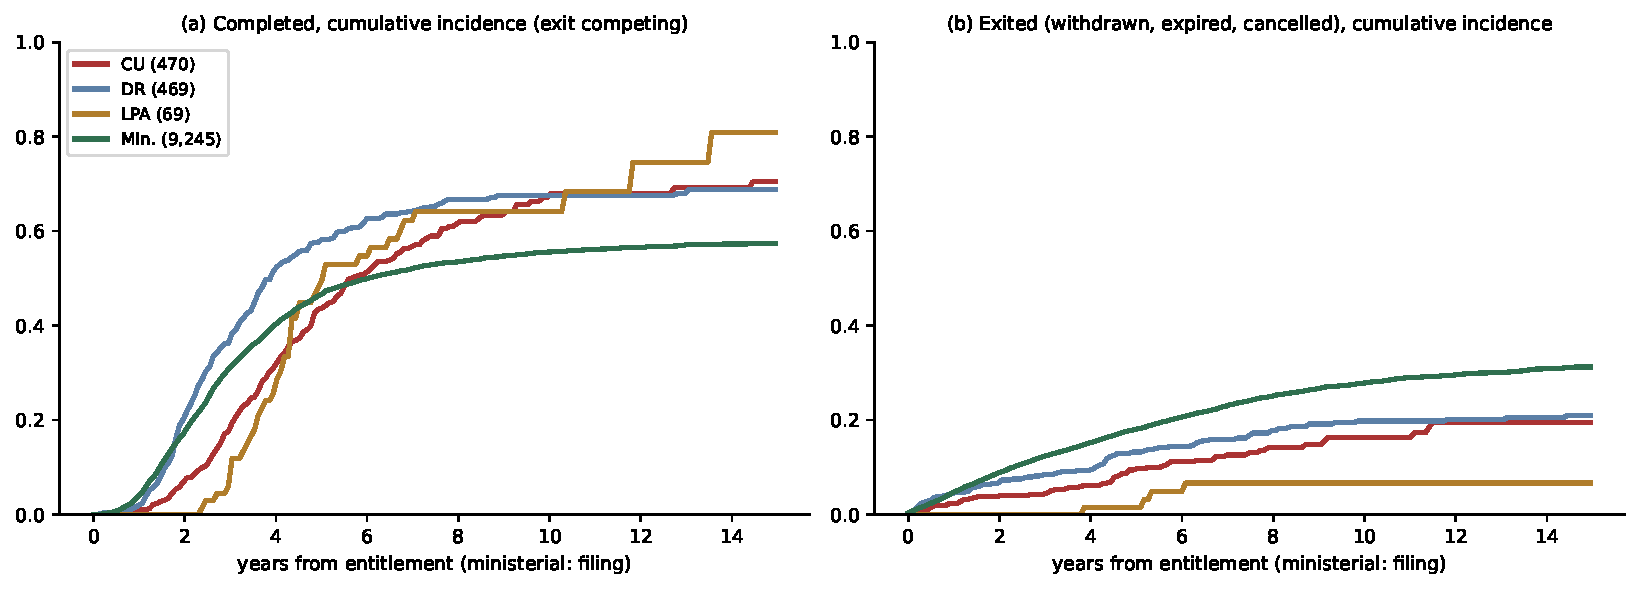
\includegraphics[width=\textwidth]{figures/fig_outcomes.pdf}
\caption{Cumulative incidence of completion (a) and of exit (b) by years from entitlement,
housing projects, every cohort; the legend gives the number of projects.}\label{fig:outcomes}
\end{figure}

\paragraph{Most entitled housing is built; a large minority is not.} Of the housing
projects entitled \ocMatureFrom--\ocMatureTo, \ocDoneCu\% of conditional uses, \ocDoneDr\% of
DRs, \ocDoneLpa\% of large project authorisations and \ocDoneMin\% of ministerial permits record
a completion; \ocExitCu\%, \ocExitDr\%, \ocExitLpa\% and \ocExitMin\% exited, and the rest are
still open. Over every cohort, the cumulative incidence of completion within \ocYears\ years is
\ocCifCu\%, \ocCifDr\%, \ocCifLpa\% and \ocCifMin\%: by that measure \ocNeverCu\%, \ocNeverDr\%,
\ocNeverLpa\% and \ocNeverMin\% of entitled projects have not delivered \ocYears\ years on. The median
time from entitlement to completion, among the mature projects that completed, is \ocMedYearsCu\
years for conditional uses, \ocMedYearsDr\ for DRs, \ocMedYearsLpa\ for large projects and
\ocMedYearsMin\ for ministerial permits.

\paragraph{Units.} The mature conditional-use projects were approved for \ocUnitsApprCu\ net
units and Housing Production records \ocUnitsHpCu\ completed on their principal permits
(\ocUnitsShareCu\%); large project authorisations \ocUnitsApprLpa\ and \ocUnitsHpLpa\
(\ocUnitsShareLpa\%); ministerial permits \ocUnitsApprMin\ and \ocUnitsHpMin\ (\ocUnitsShareMin\%).
A completion recorded under another of the project's permit numbers --- an addendum, a second
building --- is missed, so the unit shares are lower bounds; the gap is widest on the ministerial
track, where the principal permit is the only one this frame follows.

\paragraph{By parcel value.} Within tracks the completion share varies across value quintiles
without a monotone pattern (\ocDoneLoCu\% in the lowest valued quintile shown against
\ocDoneHiCu\% in the highest for conditional uses; \ocDoneLoMin\% against \ocDoneHiMin\% for
ministerial permits); cells are small on the Commission tracks.

\paragraph{What the chain cannot see.} DBI's first construction document is recorded for
\ocFcdCover\% of the mature projects, so the chain's middle link is not reliable and is shown only
as a share. Housing Production begins in \ocMatureFrom; completions before it rest on DBI's own
date. And ``entitled'' is the Commission's approving action: a project that dies before its
hearing, or is never filed, is not in the frame --- the deterred-development problem that the
risk set is meant to handle.

% ═══════════════════════════════════════════════════════════════════════════
\section{Established, and not established}

\textbf{Established.}
\begin{enumerate}
\item The full distribution --- ten percentiles and moments, and Kaplan--Meier quantiles --- of six
clocks on four tracks, by units, parcel value, period and neighbourhood, written as a table the
model can be fitted to.
\item Dispersion is large on every clock: the CV of the completed developer's clock is
\ckTotCvCu\ (conditional use), \ckTotCvDr\ (DR), \ckTotCvLpa\ (large projects) and \ckTotCvMin\
(ministerial).
\item The pre-hearing wait and the permit carry the time; most cases are decided at their first
hearing.
\item Across parcel-value quintiles the CV of the developer's clock does not fall consistently
on any track.
\item Of housing projects entitled \ocMatureFrom--\ocMatureTo, \ocDoneCu\% (conditional use) to
\ocDoneMin\% (ministerial) record a completion; the cumulative incidence of completion within
\ocYears\ years, with exit competing, is \ocCifCu\% to \ocCifMin\%.
\end{enumerate}

\textbf{Not established.}
\begin{enumerate}
\item The upper tail of the developer's clock. About a third of spells record no completion
within ten years; whether they were abandoned or finished unrecorded is a question for DBI's
data, and until it is answered the dispersion reported is that of completed projects.
\item Anything about $\sigma$ as the model defines it: ex-ante uncertainty conditional on the
developer's information. A cross-sectional CV is an upper bound on it only if the cells hold the
developer's information fixed, which they do not.
\item The CV--value relation net of period and project size, which needs a joint model, not
one-way cuts.
\item Whether the DR track's loosely falling CV is real: five quintiles, a rank correlation of
\ckCvRhoDr.
\item The share of approved units built: the unit counts miss completions recorded under a
project's other permit numbers, and are lower bounds.
\end{enumerate}

% ═══════════════════════════════════════════════════════════════════════════
\section{Reproducing this}
\label{sec:repro}

\begin{verbatim}
python analyze_permit_content.py fetch     # DBI Building Permits, every column
python analyze_permit_content.py report    # permits memo; linkage cache
python analyze_permit_content.py clocks    # this memo
python analyze_permit_content.py outcomes  # the outcome chain
\end{verbatim}

\texttt{clocks} reads the permit table, the linkage tiers (cached beside the DBI file by
\texttt{report}), the item table, the Planning records and the assessor's roll, and writes
\texttt{\$MFHR\_DATA\_ROOT/external/clocks/clocks.parquet} (one row per unit, every clock's
duration and event flag and every cut), \texttt{clock\_moments.csv} (every cell), the three
figures, one table file per table and \texttt{tables/clocks\_macros.tex}. The Kaplan--Meier
estimator and the hazard are implemented in the script (\texttt{km}, \texttt{km\_hazard}); the
project has no survival library.

\appendix
\section{The clocks, defined}
\label{sec:defs}

\begin{itemize}
\item \textbf{Application to first hearing}: from the application (the earliest entitlement
record of the case, by case number and else by stem; on the DR track, the DBI filing of the permit
under review) to the first hearing of the case. Censored at retrieval.
\item \textbf{First hearing to final action}: from the first hearing to the first hearing
recording a disposition that ends the case. Censored at retrieval.
\item \textbf{Permit filed to issued}: DBI filing to issuance of the case's permit (or of the
ministerial permit). Censored at the permit's expiry, withdrawal or other exit, else at retrieval.
\item \textbf{Final action to permit issued}: from the final action to the permit's issuance.
Censored as above.
\item \textbf{Permit issued to completion}: issuance to DBI's completion date. Censored as above.
\item \textbf{First filing to completion}: from the earlier of the application and the permit
filing to the permit's completion --- the developer's clock. Censored as above.
\end{itemize}

\end{document}
